\documentclass[12pt, a4paper]{article}

%%%%%%%%%%%%%%%紙張大小設定%%%%%%%%%%%%%%%
% \paperwidth=65cm
% \paperheight=160cm

%%%%%%%%%%%%%%%引入Package%%%%%%%%%%%%%%%
\usepackage[margin=1cm]{geometry} % 上下左右距離邊緣2cm
\usepackage{mathtools,amsthm,amssymb} % 引入 AMS 數學環境
\usepackage{yhmath}      % math symbol
\usepackage{graphicx}    % 圖形插入用
\usepackage{fontspec}    % 加這個就可以設定字體
\usepackage{type1cm}	 % 設定fontsize用
\usepackage{titlesec}   % 設定section等的字體
\usepackage{titling}    % 加強 title 功能
\usepackage{fancyhdr}   % 頁首頁尾
\usepackage{tabularx}   % 加強版 table
\usepackage[square, comma, numbers, super, sort&compress]{natbib}
% cite加強版
\usepackage[unicode, pdfborder={0 0 0}, bookmarksdepth=-1]{hyperref}
% ref加強版
\usepackage[usenames, dvipsnames]{color}  % 可以使用顏色
\usepackage[shortlabels, inline]{enumitem}  % 加強版enumerate
\usepackage{xpatch}

\graphicspath{ {images/} }
% \usepackage{tabto}      % tab
% \usepackage{soul}       % highlight
% \usepackage{ulem}       % 字加裝飾
\usepackage{wrapfig}     % 文繞圖
%\usepackage{lipsum}
% \usepackage{floatflt}    % 浮動 figure
\usepackage{float}       % 浮動環境
% \usepackage{caption}    % caption 增強
% \usepackage{subcaption}    % subfigures
% \usepackage{setspace}    % 控制空行
% \usepackage{mdframed}   % 可以加文字方框
% \usepackage{multicol}   % 多欄
% \usepackage[abbreviations]{siunitx} % SI unit
% \usepackage{dsfont}     % more mathbb

%%%%%%%%%%%%%%%%%%%TikZ%%%%%%%%%%%%%%%%%%%%%%
% \usepackage{tikz}
% \usepackage{circuitikz}

%%%%%%%%%%%%%%中文 Environment%%%%%%%%%%%%%%%
\usepackage[CheckSingle, CJKmath]{xeCJK}  % xelatex 中文
\usepackage{CJKulem}	% 中文字裝飾
\setCJKmainfont{Source Han Sans}
% 設定中文為系統上的字型,而英文不去更動,使用原TeX字型

% \XeTeXlinebreaklocale "zh"             %這兩行一定要加,中文才能自動換行
% \XeTeXlinebreakskip = 0pt plus 1pt     %這兩行一定要加,中文才能自動換行

%%%%%%%%%%%%%%%字體大小設定%%%%%%%%%%%%%%%
% \def\normalsize{\fontsize{10}{15}\selectfont}
% \def\large{\fontsize{40}{60}\selectfont}
% \def\Large{\fontsize{50}{75}\selectfont}
% \def\LARGE{\fontsize{90}{20}\selectfont}
% \def\huge{\fontsize{34}{51}\selectfont}
% \def\Huge{\fontsize{38}{57}\selectfont}

%%%%%%%%%%%%%%%Theme Input%%%%%%%%%%%%%%%%
% \input{themes/chapter/neat}
% \input{themes/env/problist}

%%%%%%%%%%%titlesec settings%%%%%%%%%%%%%%
% \titleformat{\chapter}{\bf\Huge}
            % {\arabic{section}}{0em}{}
% \titleformat{\section}{\centering\Large}
            % {\arabic{section}}{0em}{}
% \titleformat{\subsection}{\large}
            % {\arabic{subsection}}{0em}{}
% \titleformat{\subsubsection}{\bf\normalsize}
            % {\arabic{subsubsection}}{0em}{}
% \titleformat{command}[shape]{format}{label}
            % {編號與標題距離}{before}[after]

%%%%%%%%%%%%variable settings%%%%%%%%%%%%%%
% \numberwithin{equation}{section}
% \setcounter{secnumdepth}{4}  %章節標號深度
% \setcounter{tocdepth}{1}  %目錄深度
% \setcounter{section}{0}  %section 起始 counter
% \graphicspath{{images/}}  % 搜尋圖片目錄

%%%%%%%%%%%%%%%頁面設定%%%%%%%%%%%%%%%
\newcolumntype{C}[1]{>{\centering\arraybackslash}p{#1}}
\setlength{\headheight}{15pt}  %with titling
\setlength{\droptitle}{-2cm} %title 與上緣的間距
% \posttitle{\par\end{center}} % title 與內文的間距
\parindent=12pt %設定縮排的距離
% \parskip=1ex  %設定行距
% \pagestyle{empty}  % empty: 無頁碼
% \pagestyle{fancy}  % fancy: fancyhdr

% use with fancygdr
% \lhead{\leftmark}
% \chead{}
% \rhead{}
% \lfoot{}
% \cfoot{}
% \rfoot{\thepage}
% \renewcommand{\headrulewidth}{0.4pt}
% \renewcommand{\footrulewidth}{0.4pt}

% \fancypagestyle{firststyle}
% {
  % \fancyhf{}
  % \fancyfoot[C]{\footnotesize Page \thepage\ of \pageref{LastPage}}
  % \renewcommand{\headrule}{\rule{\textwidth}{\headrulewidth}}
% }

%%%%%%%%%%%%%%%重定義一些command%%%%%%%%%%%%%%%
\renewcommand{\contentsname}{目錄}  %設定目錄的標題名稱
\renewcommand{\refname}{參考資料}  %設定參考資料的標題名稱
\renewcommand{\abstractname}{\LARGE Abstract} %設定摘要的標題名稱

%%%%%%%%%%%%%%%特殊功能函數符號設定%%%%%%%%%%%%%%%
\DeclarePairedDelimiter{\abs}{\lvert}{\rvert}
\DeclarePairedDelimiter{\norm}{\lVert}{\rVert}
\DeclarePairedDelimiter{\inpd}{\langle}{\rangle} % inner product
\DeclarePairedDelimiter{\ceil}{\lceil}{\rceil}
\DeclarePairedDelimiter{\floor}{\lfloor}{\rfloor}
\DeclareMathOperator{\adj}{adj}
\DeclareMathOperator{\sech}{sech}
\DeclareMathOperator{\csch}{csch}
\DeclareMathOperator{\arcsec}{arcsec}
\DeclareMathOperator{\arccot}{arccot}
\DeclareMathOperator{\arccsc}{arccsc}
\DeclareMathOperator{\arccosh}{arccosh}
\DeclareMathOperator{\arcsinh}{arcsinh}
\DeclareMathOperator{\arctanh}{arctanh}
\DeclareMathOperator{\arcsech}{arcsech}
\DeclareMathOperator{\arccsch}{arccsch}
\DeclareMathOperator{\arccoth}{arccoth}
\newcommand{\np}[1]{\\[{#1}] \indent}
\newcommand{\transpose}[1]{{#1}^\mathrm{T}}
%%%% Geometry Symbol %%%%
\newcommand{\degree}{^\circ}
\newcommand{\Arc}[1]{\wideparen{{#1}}}
\newcommand{\Line}[1]{\overleftrightarrow{{#1}}}
\newcommand{\Ray}[1]{\overrightarrow{{#1}}}
\newcommand{\Segment}[1]{\overline{{#1}}}

%%%%%%%%%%%%%%%證明、結論、定義等等的環境%%%%%%%%%%%%%%%
\renewcommand{\proofname}{\bf 證明:} %修改Proof 標頭
\newtheoremstyle{mystyle}% 自定義Style
  {6pt}{15pt}%       上下間距
  {}%               內文字體
  {}%               縮排
  {\bf}%            標頭字體
  {.}%              標頭後標點
  {1em}%            內文與標頭距離
  {}%               Theorem head spec (can be left empty, meaning 'normal')

% 改用粗體,預設 remark style 是斜體
\theoremstyle{mystyle}	% 定理環境Style
\newtheorem{theorem}{定理}
\newtheorem{definition}{定義}
\newtheorem{formula}{公式}
\newtheorem{condition}{條件}
\newtheorem{supposition}{假設}
\newtheorem{conclusion}{結論}
\newtheorem{corollary}{推論}
\newtheorem{lemma}{引理}
\newtheorem{property}{性質}

\titlespacing*{\section} {0pt}{0ex}{0ex}

%%%%%%%%%%%%%%%Title%%%%%%%%%%%%%%%
\renewcommand{\thefootnote}{\fnsymbol{footnote}}
\title{MLDS 2017 Spring HW4 - Seq2Seq + Reinforcement Learning}
\author{B03901056 孫凡耕 B03901070 羅啟心\\
        B03901032 郭子生 B03901003 許晉嘉}
\date{\vspace{-5ex}}

\begin{document}
\maketitle 
\pagenumbering{gobble}% Remove page numbers (and reset to 1)
\thispagestyle{empty}
\section{Environment}
%\begin{enumerate}
  %\item 硬體資訊: \\
  \begin{table}[h]
  \centering
    \begin{tabular}{|C{4cm}|C{2.5cm}|C{3cm}|C{2.5cm}|C{3cm}|}
      \hline
      OS & CPU & CPU Memory & GPU & GPU Memory \\
      \hline
      \texttt{Arch linux 4.10} &
      \texttt{i7 3.6 GHz} &
      \texttt{32 GB} &
      \texttt{GTX 1080 Ti}  &
      \texttt{11 GB}  \\
      \hline
    \end{tabular}
  \end{table}
%\end{enumerate}
% End of Environment


\section{Data Sets}
\begin{itemize}
  \item Open subtitles(\href{http://opus.lingfil.uu.se/download.php?f=OpenSubtitles/en.tar.gz}{\url{http://opus.lingfil.uu.se/download.php?f=OpenSubtitles/en.tar.gz}})
  \item Movie subtitles(\href{http://www.mpi-sws.org/~cristian/Cornell_Movie-Dialogs_Corpus.html}{\url{http://www.mpi-sws.org/~cristian/Cornell_Movie-Dialogs_Corpus.html}})
\end{itemize}
% End of Data Sets


\section{Model description}
\begin{enumerate}
\item Seq2Seq 模型:\\
典型的 encoder-decoder 的模型,也就是利用 LSTM 把不同長度的輸入,
轉化為固定大小的 state,然後將此 state 傳遞給另個 LSTM,並依序輸
出當前最佳解直到遇到 \texttt{<eos>} 爲止。\\
模型所使用的參數如下:
\begin{itemize}
  \item learning rate = 0.5
  \item learning rate decay factor = 0.99
  \item max gradient norm = 5.0
  \item batch size = 64
  \item vocab size = 100000
  \item size of each model layer = {256, 512, 1024}
  \item number of layers = 4
\end{itemize}
\item Reinforment Learning 模型: \\
  我們的模型參考自 Adversarial Learning for Neural Dialogue Generation 
  \footnote{Jiwei Li, 2017, Adversarial Learning for Neural Dialogue Generation}
  這篇 paper,並改寫自該篇 paper 所提供的程式
  \footnote{https://github.com/liuyuemaicha/Adversarial-Learning-for-Neural-Dialogue-Generation-in-Tensorflow}
  ,模型所使用的參數如下:
\begin{enumerate}
  \item Generator 與 Discriminator update 的比例爲
    Generator 一次及 Discriminator 四次。
  \item Generator:
    大部分參與與上方 Seq2Seq 相同。
    \begin{itemize}
    \item dropout = 0.5
    \end{itemize}
  \item Disciminator:
    \begin{itemize}
    \item Hierarchical encoder\footnote{Jiwei Li, 2015, A Hierarchical Neural Autoencoder for Paragraphs and Documents}
    \item size per layer = 512
    \item number of layers = 4
    \item learning rate = 0.2
    \item dropout = 0.5
    \item max gradient norm = 5
    \end{itemize}
  \item Reward function:
    跟 GAN 的概念一樣,Generator 讀進來一個句子之後,會產生
    相對應的回答,Discriminator 再根據回答計算有多少機率是人
    或機器所產生的句子,若某個回答越接近人所產生的句子,則
    reward 越接近 1,反之,則越接近 0。

    以 x 表示前兩句話,y 表示 Generator 所產生的句子,以
    $Q_+(\{x,y\})$ 表示爲人所產生的機率。則 reward function
    爲 $J(\theta) = \mathbb{E}_{y \sim p(y|x)}(Q_+(\{x, y\})|\theta) $。
    則以 likelihood ratio trick 近似後可得
    $\Delta J(\theta) \approx [Q_+(\{x,y\})-b(\{x,y\})] \Delta 
    \sum\limits_t \log p(y_t|x,y_{1:t-1})$。

    此外,爲了增加 reward 對於 Generator 的影響,對於 Generator
    所產生的每個子句,都會以蒙地卡羅搜尋五次,以五次的平均作爲
    這個子句的 reward。最後,爲了讓 Generator 能持續產生好的句子,
    而不是突然找不到好的方向,每次 update 完 Discriminator 及
    Generator 後,還會在 true data 上對 Generator 進行 update
    (Teacher forcing)。
\end{enumerate}
\end{enumerate}
% End of Model description

\section{Improvement}
\begin{enumerate}
\item 在 Seq2Seq 模型中,我們嘗試在相同的 data set 之下,去調整模型的大小,
  也就是每層 layer 中所含的 cell 數量,對於不同 cell 數量,perplexity 下降
  的速度可以從 Figure~\ref{fig:movie-per} 以及 Figure~\ref{fig:open-per} 
  中看出。對於相同的 data set,如果一層的 cell 數量越多,所能蘊含的資訊量
  便越多,因此 cell 數量越多的情況下,perplexity 下降的速度便會越快。也就是說,
  模型中的大小越大,訓練的速度也會較爲快速。
  \begin{figure}[!htb]
    \centering
    \minipage{0.5\textwidth}
    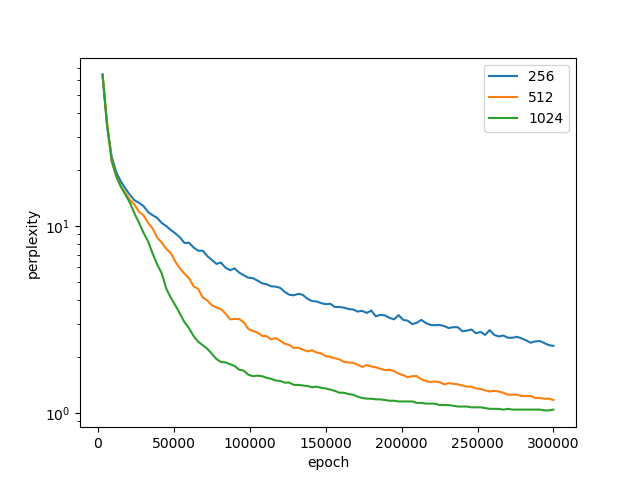
\includegraphics[scale=0.5]{movie_per.png}
    \caption{以 Movie subtitles 作爲 data set}
    \label{fig:movie-per}
   \endminipage
   \hfill
    \minipage{0.5\textwidth}
    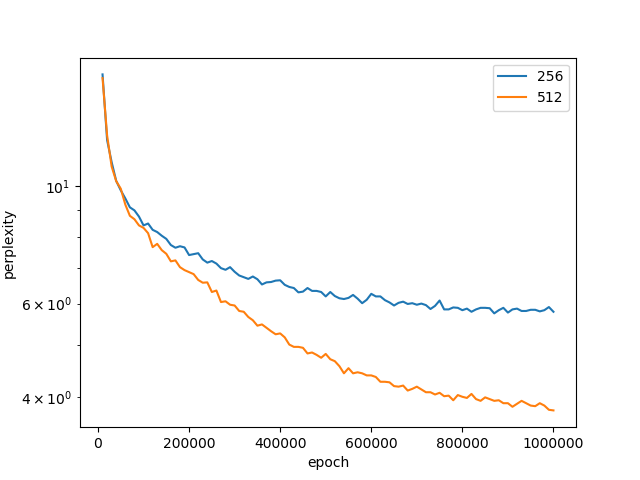
\includegraphics[scale=0.5]{open_per.png}
    \caption{以 Open subtitles 作爲 data set}
    \label{fig:open-per}
   \endminipage
  \end{figure}
\item 我們以 movie subtitles 作爲 data set 時,將太短(少於三個字)以及
  太長(長於四十個字)的句子先刪除,以及出現特殊符號(非字母數字)的句子也剔除,
  之後便剩下約莫 12 萬句對,大約剩下原先的一半。同時將單字量調整至三萬及五萬,
  所訓練出來的結果如下:\\
  \begin{tabular}{lll}
    \hline
    單字量              & 30000                    & 50000 \\
    \hline
    \hline
    how are you?        & hello , secure .         & fine . domestic .\\
    \hline
    how old are you?    & I 'm a little nervous .  & gibarian . buckle wallace .\\
    \hline
    Where are you from? & my room 's here .        & she 's a lawyer owen owen \\
    \hline
    What's your name?   & you know my name .       & gibarian fidget .\\
    \hline
    Sounds great!       & what 's he got ?         & muskets . buckle jeff .\\
    \hline
    Looks funny!        & I 've got a trunk        & i dined to see.\\
    \hline
    What's that?        & half-red , half-black -- & denning 's log .\\
    \hline
  \end{tabular} \\
  從上表可以看出,將短的句子去掉,可以使輸出更爲有趣,將長的句子去掉,可以加速
  訓練的過程,但由於句子的減少,單字量也必須減少,否則,會使模型無法訓練起來。

\item 在 Reinforcement Learning 的模型中,雖然我們所參考的 paper
  \footnote{Jiwei Li, 2017, Adversarial Learning for Neural Dialogue Generation}
  中表示,Discriminator 與 Generator 更新的比例爲 5:1,但是我們發現
  Generator 更新次數較多有利於讓 Generator 回答的結果較爲符合。
  這是由於每次更新 Generator 都會做 Teacher Forcing,因此能使 Generator
  產生更爲合理的句子。 \\
  \begin{tabular}{lll}
    \hline
    輸入句子            & 輸出回應         \\
    \hline
    \hline
    how are you?        &  fine , macaulay .            \\
    \hline                                            
    how old are you?    &  i 'm thirty-seven .         \\
    \hline                                            
    Where are you from? &  my russian \_UNK .          \\
    \hline                                            
    What's your name?   &  someone else . called me . \\
    \hline                                            
    Sounds great!       &  he 's eating the realm !   \\
    \hline                                            
    Looks funny!        &  you once you 're onto .    \\
    \hline                                            
    What's that?        &  half-red , half-black --   \\
    \hline   
  \end{tabular}
\end{enumerate}
% End of Improvement

\section{Experiment}
\begin{enumerate}
\item 在 Seq2Seq 模型中,我們實驗將相同 data set 相同模型下,不同 perplexity 時,
  模型所作出的回應如下:
  \begin{enumerate}
  \item data set 爲 movie subtitles 、模型大小爲 $4 \times 512$:\\
    \begin{tabular}{cllcll}
      perp   & 輸入句子 & 輸出回應     & perp   & 輸入句子 & 輸出回應 \\
      30  & how are you?      & no .   &    10  & how are you?      & fine , fine . \\ 
          & how old are you?  & no .   &        & how old are you?  & older . \\       
          & Where are you from? & no . &        & Where are you from? & west city . \\   
      1   & how are you?      & fine , fine . \\
          & how old are you?  & twenty-eight . \\
          & Where are you from? & california . \\
    \end{tabular}
  \item data set 爲 movie subtitles 、模型大小爲 $4 \times 256$:\\
    \begin{tabular}{cllcll}
      perp   & 輸入句子 & 輸出回應       & perp   & 輸入句子 & 輸出回應 \\
      30  & how are you?      & no .           &  10  & how are you?      & i ' m fine . \\   
          & how old are you?  & i have him .   &      & how old are you?  & o . \\            
          & Where are you from? & i have him . &      & Where are you from? & california . \\ 
      1   & how are you?      & fine . \\
          & how old are you?  & thirty-five . \\
          & Where are you from? & meet me .  \\
    \end{tabular}
  \end{enumerate}
  從不同的 perplexity 之間可以看出,明顯地,perplexity 越低,所回答出的句子
  越佳,其中模型大小爲 $4 \times 512$ 的部分在 perplexity 爲 1 時,所回答出
  的句子幾乎完全可以視爲人話。但模型大小爲 $4 \times 256$ 的部分在 perplexity
  爲 1 時,仍然有若干的句子回答不佳。我們認爲這是由於模型大小較小,因此所能
  儲存的資訊量較小的緣故所致。
\item 在 Seq2Seq 模型中,我們嘗試以相同的模型,以不同的 data set 作爲訓練資料,來
  比較以不同 data set 訓練後的模型,對於同樣的問句會有如何的回答。
  (以下結果皆爲 perplexity$\le 3$ 的情況)
  \begin{enumerate}
  \item 以下爲模型大小爲 $4 \times 256$ 的結果:\\
    \begin{tabular}{lll}
      \hline
      輸入句子            & open subtitles            & movie subtitles \\
      \hline
      \hline
      how are you?        & i ' m fine .              & fine . \\
      \hline
      how old are you?    & 00 .                      & thirty-five . \\
      \hline
      Where are you from? & i ' m from the new york . & meet me . \\
      \hline
      What's your name?   & i ' m your name .         & star . \\
      \hline
      Sounds great!       & what ?                    & yeah , i got it ! \\
      \hline
      Looks funny!        & you ' re a good man .     & is this your shovel and your husband ? \\
      \hline
      What's that?        & what ?                    & what ? \\
      \hline
    \end{tabular}
  \item 以下爲模型大小爲 $4 \times 512$ 的結果:\\
    \begin{tabular}{lll}
      \hline
      輸入句子            & open subtitles            & movie subtitles \\
      \hline
      \hline
      how are you?        & good .                    & fine , fine . \\
      \hline
      how old are you?    & 00 .                      & twenty-eight . \\
      \hline
      Where are you from? & you ' re from texas .     & southern california . \\
      \hline
      What's your name?   & you know what ?           & lisette . \\
      \hline
      Sounds great!       & no .                      & let ' s get out of here . \\
      \hline
      Looks funny!        & you know what ?           & what ? \\
      \hline
      What's that?        & what ?                    & what do you mean ? \\
      \hline
    \end{tabular}
  \end{enumerate}
  從以上的結果可以看出,在模型大小不夠大的時候,以 open subtitles 及
  movie subtitles 爲 data set 的結果相去不遠,又以 open subtitles 的部分
  較爲像人所作出的回應。但將模型大小擴大之後,可以看出 open subtitles 的
  部分並沒有顯著的進步,因此可以推斷出 open subtitles 的資料量也許較爲簡單
  ,而將模型擴大之後,movie subtitles 的結果便有十分顯著的進步,幾乎所有的
  回應都有相當程度的貼近人話。可以推斷,movie subtitles 的資訊量較爲完整
  ,但也需要較大的模型。
\item 在 Reinforcement Learning 的部分,由於我們 data 的量並不夠多,
  加上 model pretrained 的部分也不夠多,以及我們的 RL model 是基於前兩句
  來推測下一句,但實際上我們的資料是一句對一句,因此,模型實際上並不太正確。
  而且當 Discriminator 更新次數比較少的時候,便會出現答非所問的現象,
  這個現象在訓練越久便會越明顯!下表爲 Reinforcement Learning Generate 更新
  次數與 Discriminator 更新次數爲 1:1 時的結果。 \\
  \begin{tabular}{lll}
    \hline
    輸入句子            & 輸出回應        \\
    \hline
    \hline
    how are you?        & head for bridge .          \\
    \hline
    how old are you?    & i didn't see her .         \\
    \hline
    Where are you from? & my russian boys .          \\
    \hline
    What's your name?   & william simpson . robert rath . \\
    \hline
    Sounds great!       & sally , kitchen .            \\
    \hline
    Looks funny!        & i 'm sorry ... lee lother 's a very ...     \\
    \hline
    What's that?        & i 'm getting . \\
    \hline
  \end{tabular}
\item 因爲 Generator 與 Discriminator 需要保持平衡的狀態,我們
  所訓練出來的模型,所觀察到的 Reward per sentence 大致上維持在
  0.4 左右。然而,如果去掉 Teacher Focing,則 Generator
  即使在有 pretrain 的情況下,仍然很難獲得 Reward。
  如 Figure~\ref{fig:tf} 所示,Reward 基本都維持一致。
  但不確定原因爲何如 Figure~\ref{fig:tl} 所示 Teacher Loss
  會上升。
  \begin{figure}[!htb]
    \centering
    \minipage{0.5\textwidth}
    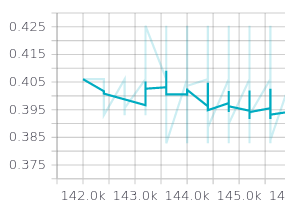
\includegraphics[scale=0.5]{tf.png}
    \caption{Reward}
    \label{fig:tf}
   \endminipage
   \hfill
    \centering
    \minipage{0.5\textwidth}
    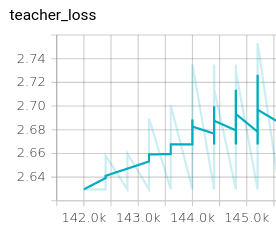
\includegraphics[scale=0.5]{tl.png}
    \caption{Teacher Loss}
    \label{fig:tl}
   \endminipage
  \end{figure}
\end{enumerate}
% End of Experiment

\section{Team division}
\begin{table}[h]
\centering
\begin{tabular}{ |C{2cm}|C{10cm}| }
  \hline
  孫凡耕 & RL、分配組內工作、教導組員\\
  \hline
  羅啟心 & 協助餘項事務\\
  \hline
  郭子生 & 協助餘項事務 \\
  \hline
  許晉嘉 & Seq2Seq、統整撰寫報告、跑實驗 \\
  \hline
\end{tabular}
\end{table}
% End of Team division

\end{document}
